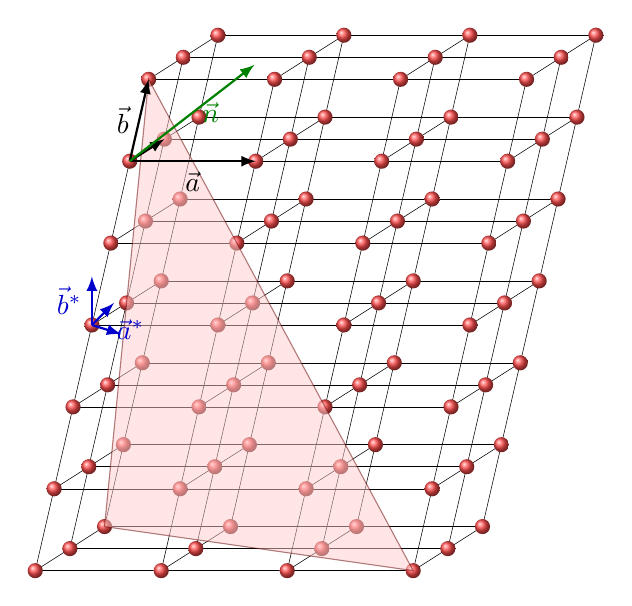
\begin{tikzpicture}[x  = {(1cm,0cm)},
  y  = {(0cm,1cm)},
  z  = {(0.35cm,0.35cm)},
  scale = 0.8]

  % direct lattice constants
  \def\dax{2}
  \def\day{0.3}
  \def\daz{0.2}
  \def\dby{1.3}

  % a = vector3d(2,0,0)
  % b = vector3d(0.3, 1.3, 0)
  % c = vector3d(0.2, 0, 1)
  % V = cdot(cross(a,b),c);
  % astar = cross(b,c) / V
  % bstar = cross(c,a) / V
  % cstar = cross(a,b) / V

  % reciprocal lattice constants


  % grid
  \foreach \y in {0,1,...,6}
  \foreach \z in {0,1,...,2}
  \draw[style=help lines,color=black] (\dax*0+\day*\y+\daz*\z,\dby*\y,\z)
  -- (\dax*3+\day*\y+\daz*\z,\dby*\y,\z);

  \foreach \x in {0,1,...,3}
  \foreach \z in {0,1,...,2}
  \draw[style=help lines,color=black] (\dax*\x+\day*0+\daz*\z,\dby*0,\z)
  -- (\dax*\x+\day*6+\daz*\z,\dby*6,\z);

  \foreach \x in {0,1,...,3}
  \foreach \y in {0,1,...,6}
  \draw[style=help lines,color=black] (\dax*\x+\day*\y+\daz*0,\dby*\y,0)
  -- (\dax*\x+\day*\y+\daz*2,\dby*\y,2);

  % path to vector h
  % \draw[->, >=latex, ultra thick, color=green, style=dashed] (0,0,0) ->
  % +(\dax*3,0,0) -> +(\dax*3+\daz*1,0,1) -> (\dax*3+\day*2+\daz*1,\dby*2,1);

  % atoms
  \foreach \x in {0,1,...,3}
  \foreach \y in {0,1,...,6}
  \foreach \z in {0,1,...,2}
  {
  \shade[ball color=red!70] (\dax*\x+\day*\y+\daz*\z,\dby*\y,\z) circle (.12cm);
  }

  % lattice plane
  \filldraw[fill=red!20,draw=red!40!black,opacity=0.5] (\dax*3,0,0) --
  (\daz*2,0,2) -- (\day*6,\dby*6,0) -- cycle;

  % unit cell
  \draw[->, >=latex, thick] (5*\day,5*\dby,0) -> node[left] {$\vec{b}$}
  +(\day,\dby,0);
  \draw[->, >=latex,  thick, color=black]
  (5*\day,5*\dby,0) -> node[below] {$\vec{a}$} +(\dax,0,0);
  \draw[->, >=latex,  thick, color=black]
  (5*\day,5*\dby,0) -> +(\daz,0,1);

  % normal vector
  % n = (1/2,1,1/3) = (3,6,2)
  % a* = (0.5 -0.115385 -0.1)
  % b* = (0 0.769231 0)
  % c* = (0 0 1)

  \draw[->, >=latex, thick, color=green!50!black] (5*\day,5*\dby,0) -> node[right] {$\vec{n}$}
  +(2*0.5, -2*0.11 + 1*0.77, -2*0.1 + 3);
 %  +(h*0.5, -h*0.11 + k*0.77, -h*0.1 -k*0.038 +ell);
  \draw[->, >=latex, thick, color=blue!80!black] (3*\day,3*\dby,0) -> node[right] {$\vec{a}^{*}$}
  +(1*0.5, -1*0.11 + 0*0.77, -1*0.1);
  \draw[->, >=latex, thick, color=blue!80!black] (3*\day,3*\dby,0) -> node[left] {$\vec{b}^{*}$}
  +(0*0.5, -0*0.11 + 1*0.77, 0);

  \draw[->, >=latex, thick, color=blue!80!black] (3*\day,3*\dby,0) -> node[right] {}
   +(0*0.5, -0*0.11 + 0*0.77, 1);

\end{tikzpicture}

%%% Local Variables:
%%% mode: latex
%%% TeX-master: "../1_crystalLattice"
%%% End:
